%----------------------------------------------------------------------------------------
%	Inställningar och dokumentkonfiguration
%----------------------------------------------------------------------------------------

\documentclass[paper=a4, fontsize=11pt]{report} % A4-sida och 11 punkters fontstorlek

\usepackage[T1]{fontenc} % 8-bitarskodning som har 256 glyfer
\usepackage[swedish]{babel} % Svenskt språk
\usepackage[utf8]{inputenc} % För svenska tecken
\usepackage{dtklogos} % Logos
\usepackage{wallpaper} % Bakgrundsbild
\usepackage{fancyhdr} % Specialsidhuvud och sidfot
\usepackage{enumerate} 
\usepackage{xifthen}% provides \isempty test
\pagestyle{fancyplain} % Använd sidhuvud och sidfot på alla sidor
\fancyhead[L]{Seminar 1 -- 1DV020 -- 2015 -- Server Administration} % Titel till vänster i sidhuvud
\fancyhead[C]{} % Tomt i mitten
\fancyhead[R]{} % Tomt till höger
\fancyfoot[L]{} % Tomt till vänster
\fancyfoot[C]{} % Tomt i mitten
\fancyfoot[R]{\thepage} % Sidnumrering till höger i sidfoten
\renewcommand\thesection{\arabic{section}} % Section beter sig som i dokumentklassen article

\newcommand{\win}[1]{Microsoft Windows Server\ifthenelse{\isempty{#1}}{}{ #1}}
\newcommand{\gui}[0]{``Server with a GUI''}
\newcommand{\core}[0]{Windows Server Core}
%----------------------------------------------------------------------------------------
%	TITLE SECTION
%----------------------------------------------------------------------------------------
\newcommand\BackgroundPic{
    \put(-50,-50){
    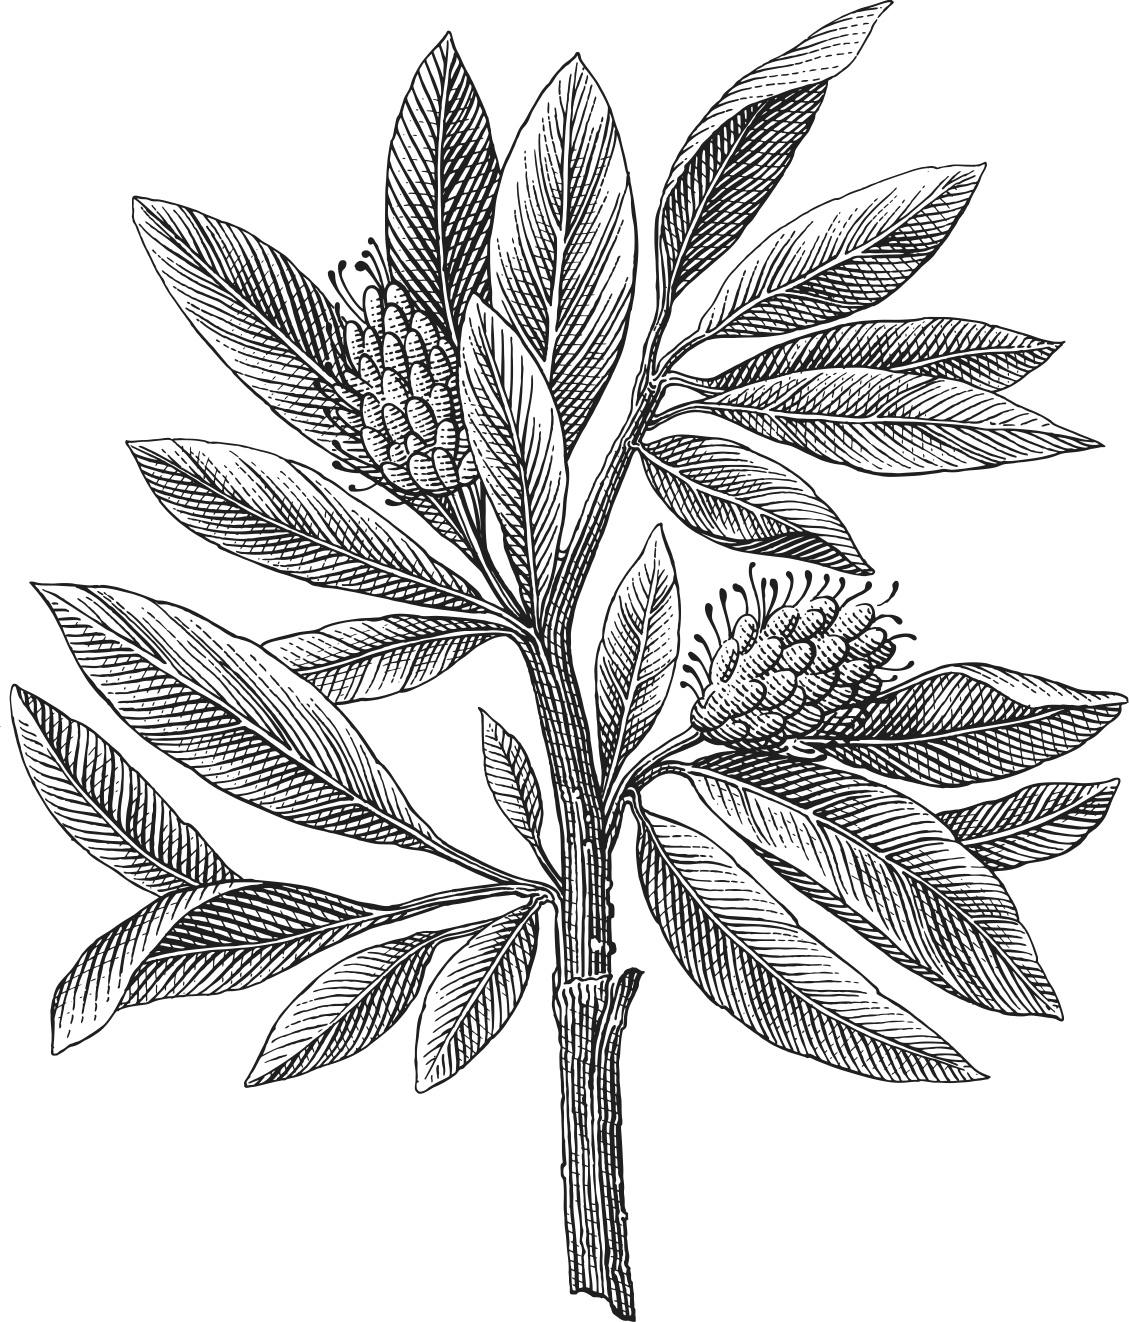
\includegraphics[keepaspectratio,scale=0.65]{lnu_etch.png} % Bakgrundsbild
    }
}
\newcommand\BackgroundPicLogo{
    \put(15,700){
    
\includegraphics[keepaspectratio,scale=0.10]{logo.png} % Logga i vänstra hörnet
    }
}

\newcommand{\horrule}[1]{\rule{\linewidth}{#1}} % Skapa hortisontell linje

\title{	\vspace{-10cm}
    \normalfont \normalsize
    \textsc{Linnaeus University} \\ [25pt] % Universitetes namn
    \horrule{0.5pt} \\[0.4cm] % Tunn linje högst upp
    \huge Seminar 1\\ % Arbetes titel
	\large \textcolor{gray}{1DV020 -- Server Administration}
    \horrule{0.5pt} \\[0.4cm] % Tunn linje längst ner
}

\author{Jacob Lindehoff} % Författarnas namn

\date{\normalsize\today} % Dagens datum

\begin{document}
\AddToShipoutPicture*{\BackgroundPic} % Lägger in backgrundsbild på första sidan
\AddToShipoutPicture*{\BackgroundPicLogo}
\maketitle % Skriv ut titeln
\noindent % Tabba inte in på första meningen

%------------------------------------------------
%	Introduktion
%------------------------------------------------
\section{Introduction}
During this seminar, we will address the following topics:
\begin{itemize}
\item Server vs. Client
\item Installation of various server operating systems
\item Basic configuration
\item Administrative Tools

\end{itemize}

%------------------------------------------------
%	Deadline
%------------------------------------------------
\section{Dealine}
The seminar is on the {\color{red}28th January 2015} and it is compulsory. If you cannot participate, it must be notified in advance and a written report of the seminar must be submitted no later than {\color{red}3 days} after the seminar. The written report should contain detailed answers to all questions in the seminar.
\newpage
%------------------------------------------------
%	Seminariefrågor
%------------------------------------------------
\section{Seminar Questions}

\begin{enumerate}
\begin{large}
\item What is it that makes a computer to a server (hardware)?
\item What is meant by a Server when talking about software?
\item What are the major historical milestones for:
    \begin{enumerate}[a.]
        \item \win{}
        \item Linux
    \end{enumerate}
\item Describe the different types of System administrator roles and which you are most interested in working as?
\item You have a client who has 50 clients, they want a new file server.
    \begin{enumerate}[a.]
        \item How do you find appropriate hardware for the company?
        \item What hardware do you recommend?
    \end{enumerate}
\item What is important to consider before installing a server operating system?
\item What is a HCL and why should it be checked before you install server operating system?
\item Client Access Licenses
    \begin{enumerate}[a.]
        \item What are the different CALs thats Microsoft has?
        \item How do tey work?
        \item How to choose the right CAL, in which scenarios dose the different CALs fit?
    \end{enumerate}
\item \core
    \begin{enumerate}[a.]
        \item What is \core?
        \item In which scenarios is a Server Core installation appropriate?
        \item What advantages does a \core{} installation compared with a \gui?
    \end{enumerate}

\end{large}
\end{enumerate}
\end{document}
